\chapter{Methodology}
\label{ch:methodology}
This section works through an example case and uses that to demonstrate how an online store may gather data on a user and thus create a profile of them to create specific, targeted content for them.


%
% Section: Example Case - Online Stores and Single Sign-On
%
\section{Example Case - Online Stores and Single Sign-On}
\label{sec:methodology:caseStudy}
In a hypothetical and not-so-distant future, Web3 technologies might reinvent how we use the internet. From alternate currencies to dApps; the future internet may not be as we know it today in its current Web2 state. A hypothetical scenario will be described in this section in order to look at how user data might be tracked in this future version of the internet.

Imagine Alice visits an online store for shoes. She does not have a profile for this website yet and sees that she can create a profile using her wallet's SSO function. After doing so, she purchases a pair of shoes. She receives a notification from the website that they would like to gift an NFT to Alice. She accepts and a digital twin of her newly bought shoe as an NFT is placed into her wallet.

A few days later, Alice visits a different online shop. She also does not have an account here and again uses the SSO function to create a profile. Her wallet is thus connected with this new website. Immediately, she receives shoe recommendations from the website that fit her exact taste.

How is the second online shop able to give specific recommendations to Alice just by having a connection set up to her wallet?


%
% Section: Public Wallet Address
%
\section{Public Wallet Address}
\label{sec:methodology:address}
In the above scenario, the user grants wallet access to the online stores. As mentioned in section \ref{sec:bg_tech:wallets}, the online stores are thus able to view the public address of the wallet. Although the stores do not know anything about the user specifically (i.e. name, age, etc.), this information alone is enough to be able to make specific recommendations to a potential buyer.

This is possible because everything written to the blockchain is public knowledge. When an online store, as in the example above, places an NFT into a user's wallet, the transaction is recorded with with both parties' public addresses.

Etherscan \cite{etherscan} and OpenSea \cite{openSea} are two popular websites for viewing transactions and profiles. When looking up a user's public address on Etherscan, every transaction associated with that public address can be viewed \cite{etherscan}. Figure \ref{fig:openSea} shows an example OpenSea profile, also viewable by anyone. OpenSea is a marketplace to view and trade NFTs \cite{openSea}. In the example, the user with the public address starting with \textit{0xd4C6}, is displayed. This user has three NFTs currently in their wallet.

This information about a user is automatically accessible to any platform that a user connects their wallet to. In the above example, the second online store would be able to see the contents of the users wallet, recognize that they have previously bought a certain shoe from another store by seeing the associated NFT. Knowing what shoe a user has previously bought, they are able to recommend similar products to the user. For example, if a customer has previously bought a certain shoe from Nike and received an NFT for their purchase, then Adidas can use the information of that NFT to recommend products of their own.

\begin{figure}[t]
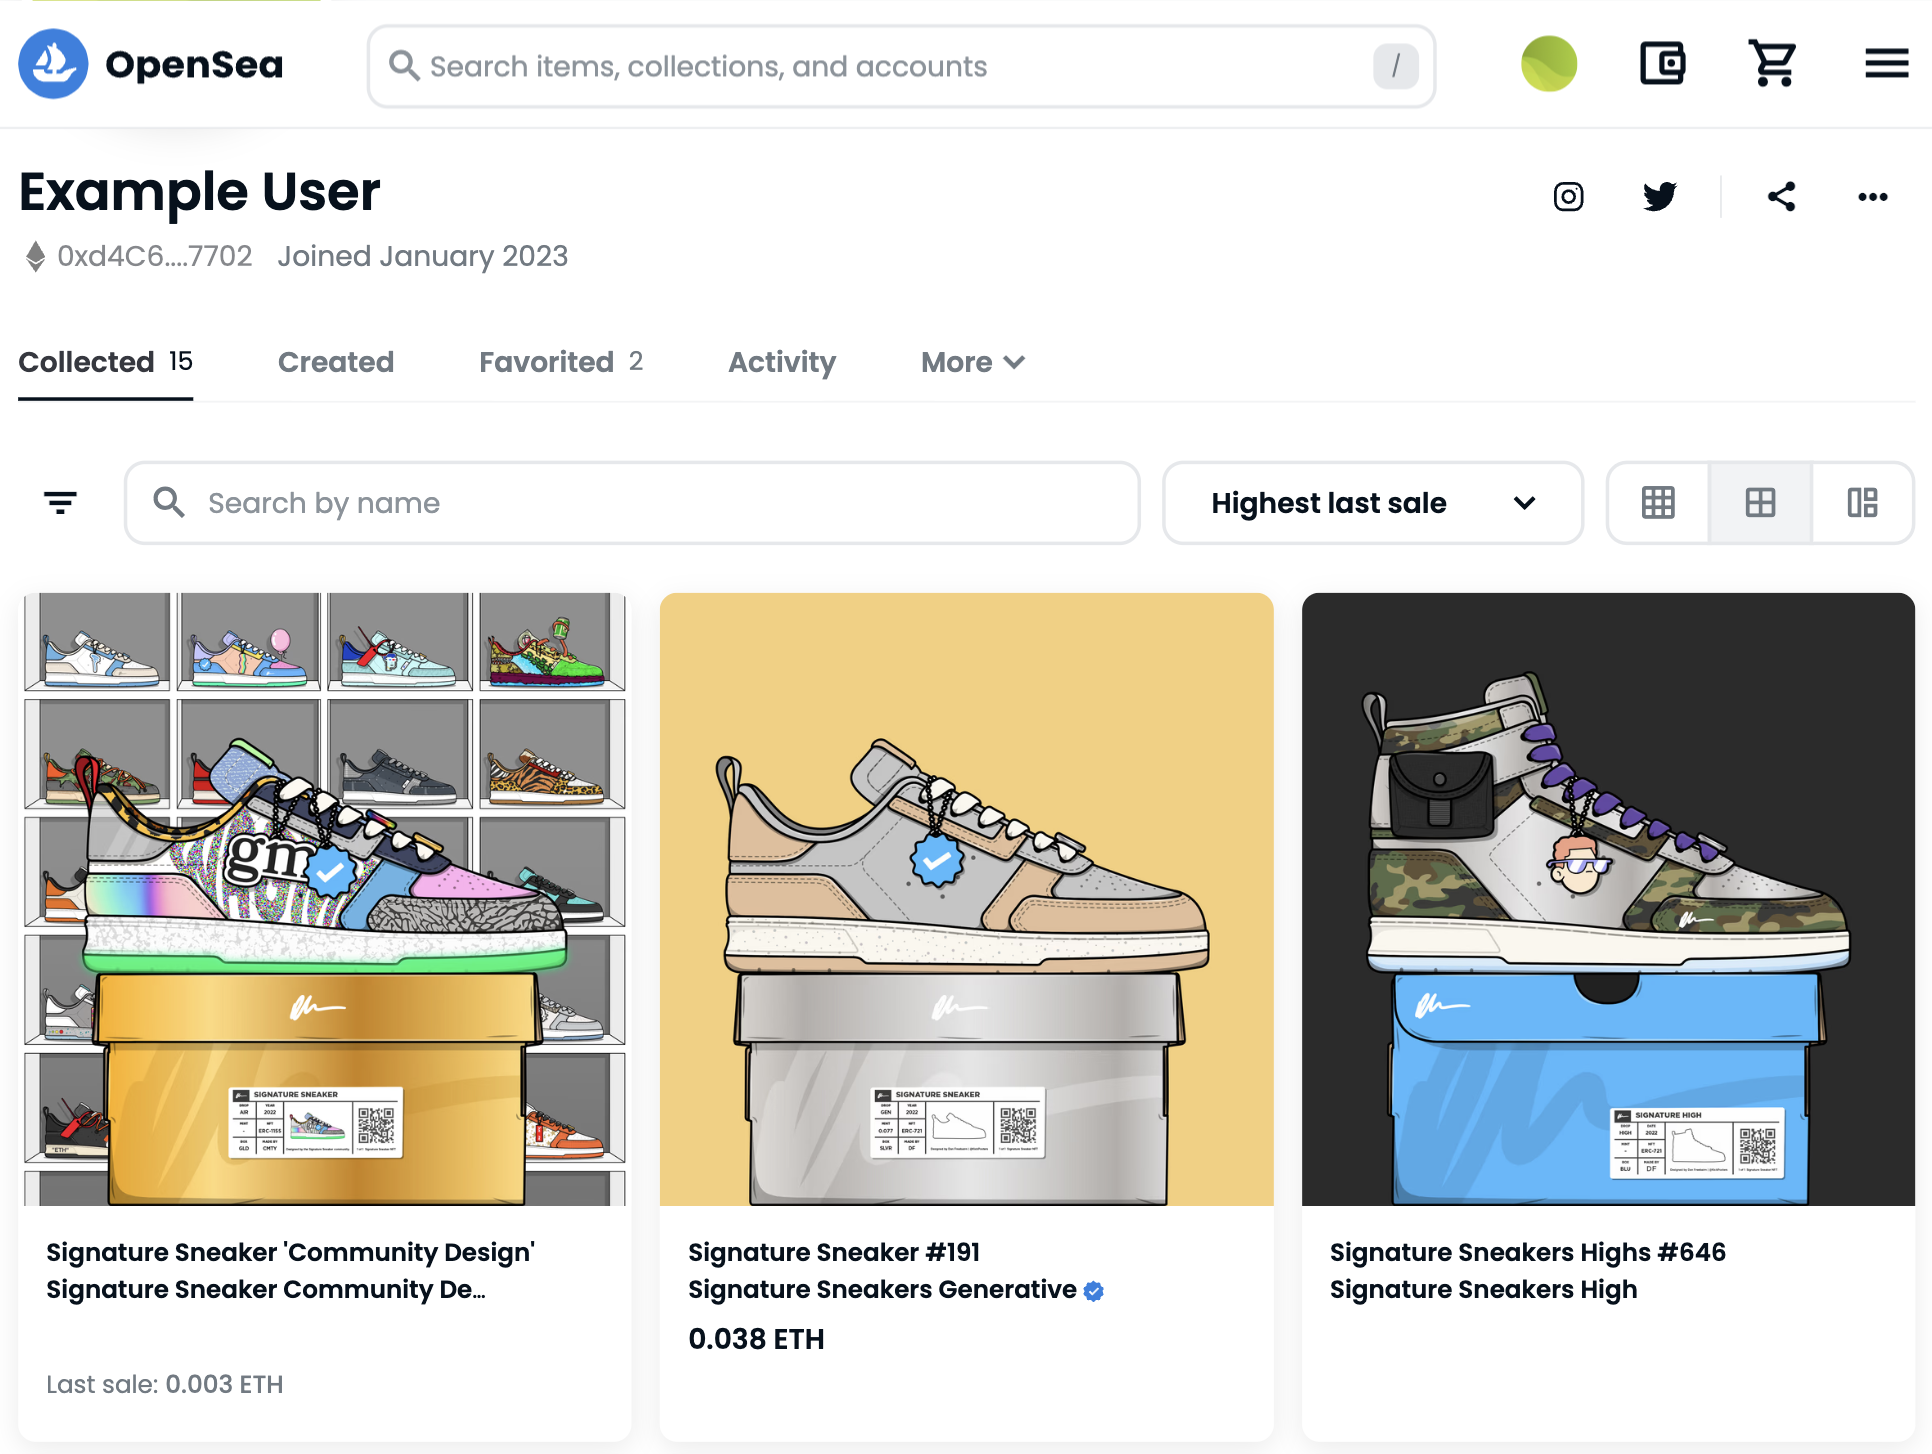
\includegraphics[width=\textwidth]{./gfx/openSea.png}
\centering
\caption{An example profile on the online NFT marketplace \textit{OpenSea} \cite{openSea}.}
\label{fig:openSea}
\end{figure}

%
% Section: Further Obtainable Data
%
\section{Further Obtainable Data}
\label{sec:methodology:moreData}

Todo: Something about transactional data that can be viewed on Etherscan. Not only can companies see our wallets and what NFTs we're holding, but they can also see who we are interacting with and can use that information to find things out about us.

Wallet Balance wird auch angezeigt



